\documentclass[twoside]{book}

% Packages required by doxygen
\usepackage{fixltx2e}
\usepackage{calc}
\usepackage{doxygen}
\usepackage[export]{adjustbox} % also loads graphicx
\usepackage{graphicx}
\usepackage[utf8]{inputenc}
\usepackage{makeidx}
\usepackage{multicol}
\usepackage{multirow}
\PassOptionsToPackage{warn}{textcomp}
\usepackage{textcomp}
\usepackage[nointegrals]{wasysym}
\usepackage[table]{xcolor}

% Font selection
\usepackage[T1]{fontenc}
\usepackage[scaled=.90]{helvet}
\usepackage{courier}
\usepackage{amssymb}
\usepackage{sectsty}
\renewcommand{\familydefault}{\sfdefault}
\allsectionsfont{%
  \fontseries{bc}\selectfont%
  \color{darkgray}%
}
\renewcommand{\DoxyLabelFont}{%
  \fontseries{bc}\selectfont%
  \color{darkgray}%
}
\newcommand{\+}{\discretionary{\mbox{\scriptsize$\hookleftarrow$}}{}{}}

% Page & text layout
\usepackage{geometry}
\geometry{%
  a4paper,%
  top=2.5cm,%
  bottom=2.5cm,%
  left=2.5cm,%
  right=2.5cm%
}
\tolerance=750
\hfuzz=15pt
\hbadness=750
\setlength{\emergencystretch}{15pt}
\setlength{\parindent}{0cm}
\setlength{\parskip}{3ex plus 2ex minus 2ex}
\makeatletter
\renewcommand{\paragraph}{%
  \@startsection{paragraph}{4}{0ex}{-1.0ex}{1.0ex}{%
    \normalfont\normalsize\bfseries\SS@parafont%
  }%
}
\renewcommand{\subparagraph}{%
  \@startsection{subparagraph}{5}{0ex}{-1.0ex}{1.0ex}{%
    \normalfont\normalsize\bfseries\SS@subparafont%
  }%
}
\makeatother

% Headers & footers
\usepackage{fancyhdr}
\pagestyle{fancyplain}
\fancyhead[LE]{\fancyplain{}{\bfseries\thepage}}
\fancyhead[CE]{\fancyplain{}{}}
\fancyhead[RE]{\fancyplain{}{\bfseries\leftmark}}
\fancyhead[LO]{\fancyplain{}{\bfseries\rightmark}}
\fancyhead[CO]{\fancyplain{}{}}
\fancyhead[RO]{\fancyplain{}{\bfseries\thepage}}
\fancyfoot[LE]{\fancyplain{}{}}
\fancyfoot[CE]{\fancyplain{}{}}
\fancyfoot[RE]{\fancyplain{}{\bfseries\scriptsize Generated by Doxygen }}
\fancyfoot[LO]{\fancyplain{}{\bfseries\scriptsize Generated by Doxygen }}
\fancyfoot[CO]{\fancyplain{}{}}
\fancyfoot[RO]{\fancyplain{}{}}
\renewcommand{\footrulewidth}{0.4pt}
\renewcommand{\chaptermark}[1]{%
  \markboth{#1}{}%
}
\renewcommand{\sectionmark}[1]{%
  \markright{\thesection\ #1}%
}

% Indices & bibliography
\usepackage{natbib}
\usepackage[titles]{tocloft}
\setcounter{tocdepth}{3}
\setcounter{secnumdepth}{5}
\makeindex

% Hyperlinks (required, but should be loaded last)
\usepackage{ifpdf}
\ifpdf
  \usepackage[pdftex,pagebackref=true]{hyperref}
\else
  \usepackage[ps2pdf,pagebackref=true]{hyperref}
\fi
\hypersetup{%
  colorlinks=true,%
  linkcolor=blue,%
  citecolor=blue,%
  unicode%
}

% Custom commands
\newcommand{\clearemptydoublepage}{%
  \newpage{\pagestyle{empty}\cleardoublepage}%
}

\usepackage{caption}
\captionsetup{labelsep=space,justification=centering,font={bf},singlelinecheck=off,skip=4pt,position=top}

%===== C O N T E N T S =====

\begin{document}

% Titlepage & ToC
\hypersetup{pageanchor=false,
             bookmarksnumbered=true,
             pdfencoding=unicode
            }
\pagenumbering{roman}
\begin{titlepage}
\vspace*{7cm}
\begin{center}%
{\Large Servocontrol }\\
\vspace*{1cm}
{\large Generated by Doxygen 1.8.11}\\
\end{center}
\end{titlepage}
\clearemptydoublepage
\tableofcontents
\clearemptydoublepage
\pagenumbering{arabic}
\hypersetup{pageanchor=true}

%--- Begin generated contents ---
\chapter{R\+E\+A\+D\+ME}
\label{md_README}
\hypertarget{md_README}{}
\section*{Hello, fellow robotics learners}

For those of us who are on a budget, have brain-\/sized balls (or ball-\/sized brains, depending on P\+OV), and/or plan to control the robot from an embedded system (or any combination thereof), I\textquotesingle{}ve been trying to implement some of the M\+A\+T\+L\+AB functionality in C.~\newline
 I\textquotesingle{}ts work in progress, dudes. Forward and reverse kinematics will be coming any day now.~\newline
 Feel free to contribute, but don\textquotesingle{}t improve \hyperlink{matrix_8c_a1e8d8c0421f716763d5bbb5c39af0e5b}{matrix\+\_\+mul()} unless you really, really, really, really know what you\textquotesingle{}re doing -\/ I pulled my hair out to make that beast work.

To compile, type make at the \$ prompt~\newline
 \$ make

\subsection*{matrix}

\hyperlink{matrix_8c}{matrix.\+c} contains enough maxtric operations to get through the course, and then adding whatever is necessary to get a Chinese 6\+D\+OF robot arm working with Tower\+Pro M\+G996R servos. The low-\/level stuff will be in \hyperlink{servoctl_8c}{servoctl.\+c}.

To use the matrix operations, include \hyperlink{matrix_8h}{matrix.\+h}. {\ttfamily  \#include \char`\"{}matrix.\+h\char`\"{}}

{\ttfamily /$\ast$ Let\textquotesingle{}s multiply two matrices, m x m2 and store the product in m3 $\ast$/}

{\ttfamily /$\ast$ 1. Declare the three matrices you\textquotesingle{}ll be using. $\ast$/ \begin{DoxyVerb}matrix_t* m = matrix_new(3,3); /* Create a 3x3 matrix */
matrix_t* m2 = matrix_new(1,3);/* Create a 1x3 matrix */
matrix_t* m3;
\end{DoxyVerb}
}

{\ttfamily /$\ast$ 2. Put some values in m and m2 $\ast$/ \begin{DoxyVerb}matrix_set_col(m,0, 1.0, 2.0, 3.0);
matrix_set_col(m,1, 4.0, 5.0, 6.0);
matrix_set_col(m,2, 7.0, 8.0, 9.0);

matrix_set_col(m2,0, 1.0, 2.0, 3.0);

/* Print it */
matrix_printf("%2.0f ", m);
printf("*\n");
matrix_printf("%2.0f ", m2);
printf("=\n");
\end{DoxyVerb}
}

{\ttfamily /$\ast$ 3. Multiply them and print the result $\ast$/ \begin{DoxyVerb}m3 = matrix_mul(m, m2);
matrix_printf("%2.0f ", m3);
\end{DoxyVerb}
}

{\ttfamily /$\ast$ 4. Clean up, and you\textquotesingle{}re done. $\ast$/ matrix\+\_\+del(m2); matrix\+\_\+del(m3);}

{\ttfamily  matrix\+\_\+del(m); }

\subsection*{Servoctl}

Contains low-\/level routines for dealing with servos and the Adafruit servo controller. 
\chapter{Bug List}
\label{bug}
\hypertarget{bug}{}

\begin{DoxyRefList}
\item[\label{bug__bug000001}%
\hypertarget{bug__bug000001}{}%
Global \hyperlink{matrix_8c_a2e2541f2040177403b95e30f38b232fe}{matrix\+\_\+rot\+\_\+x} (matrix\+\_\+t $\ast$m, double theta)]Create x,y,z static rotation matrices to avoid alloc/free
\begin{DoxyItemize}
\item The result must be deleted with \hyperlink{matrix_8c_a8277c0c702668ac9c20d5b4fbbb1c805}{matrix\+\_\+del()} 
\end{DoxyItemize}
\end{DoxyRefList}
\chapter{Data Structure Index}
\section{Data Structures}
Here are the data structures with brief descriptions\+:\begin{DoxyCompactList}
\item\contentsline{section}{\hyperlink{structmatrix}{matrix} }{\pageref{structmatrix}}{}
\end{DoxyCompactList}

\chapter{File Index}
\section{File List}
Here is a list of all files with brief descriptions\+:\begin{DoxyCompactList}
\item\contentsline{section}{\hyperlink{main_8c}{main.\+c} }{\pageref{main_8c}}{}
\item\contentsline{section}{\hyperlink{matrix_8c}{matrix.\+c} }{\pageref{matrix_8c}}{}
\item\contentsline{section}{\hyperlink{matrix_8h}{matrix.\+h} }{\pageref{matrix_8h}}{}
\item\contentsline{section}{\hyperlink{servocontrol_8c}{servocontrol.\+c} }{\pageref{servocontrol_8c}}{}
\item\contentsline{section}{\hyperlink{servoctl_8c}{servoctl.\+c} }{\pageref{servoctl_8c}}{}
\item\contentsline{section}{\hyperlink{servoctl_8h}{servoctl.\+h} }{\pageref{servoctl_8h}}{}
\item\contentsline{section}{\hyperlink{test__matrix_8c}{test\+\_\+matrix.\+c} }{\pageref{test__matrix_8c}}{}
\end{DoxyCompactList}

\chapter{Data Structure Documentation}
\hypertarget{structlinkage}{}\section{linkage Struct Reference}
\label{structlinkage}\index{linkage@{linkage}}


{\ttfamily \#include $<$servoctl.\+h$>$}

\subsection*{Data Fields}
\begin{DoxyCompactItemize}
\item 
\hyperlink{structlinkage_ab7212a9ff1ec58211f1b689374f11766}{base\+\_\+x}
\item 
\hyperlink{structlinkage_aed760843bedfbb6de7f205758ef0d49b}{base\+\_\+y}
\end{DoxyCompactItemize}


\subsection{Field Documentation}
\index{linkage@{linkage}!base\+\_\+x@{base\+\_\+x}}
\index{base\+\_\+x@{base\+\_\+x}!linkage@{linkage}}
\subsubsection[{\texorpdfstring{base\+\_\+x}{base_x}}]{\setlength{\rightskip}{0pt plus 5cm}base\+\_\+x}\hypertarget{structlinkage_ab7212a9ff1ec58211f1b689374f11766}{}\label{structlinkage_ab7212a9ff1ec58211f1b689374f11766}
\index{linkage@{linkage}!base\+\_\+y@{base\+\_\+y}}
\index{base\+\_\+y@{base\+\_\+y}!linkage@{linkage}}
\subsubsection[{\texorpdfstring{base\+\_\+y}{base_y}}]{\setlength{\rightskip}{0pt plus 5cm}base\+\_\+y}\hypertarget{structlinkage_aed760843bedfbb6de7f205758ef0d49b}{}\label{structlinkage_aed760843bedfbb6de7f205758ef0d49b}


The documentation for this struct was generated from the following file\+:\begin{DoxyCompactItemize}
\item 
\hyperlink{servoctl_8h}{servoctl.\+h}\end{DoxyCompactItemize}

\hypertarget{structmatrix}{}\section{matrix Struct Reference}
\label{structmatrix}\index{matrix@{matrix}}


{\ttfamily \#include $<$matrix.\+h$>$}

\subsection*{Data Fields}
\begin{DoxyCompactItemize}
\item 
int \hyperlink{structmatrix_a53e53380c64d2dcc85486da7f90794d5}{nrows}
\item 
int \hyperlink{structmatrix_a7c4b990ebe8d2c098f3974f6ffe0c9b4}{ncols}
\item 
double $\ast$ \hyperlink{structmatrix_a18edff6f6f8cc7071adfd9bc826378ef}{v}
\end{DoxyCompactItemize}


\subsection{Field Documentation}
\index{matrix@{matrix}!ncols@{ncols}}
\index{ncols@{ncols}!matrix@{matrix}}
\subsubsection[{\texorpdfstring{ncols}{ncols}}]{\setlength{\rightskip}{0pt plus 5cm}int ncols}\hypertarget{structmatrix_a7c4b990ebe8d2c098f3974f6ffe0c9b4}{}\label{structmatrix_a7c4b990ebe8d2c098f3974f6ffe0c9b4}
\index{matrix@{matrix}!nrows@{nrows}}
\index{nrows@{nrows}!matrix@{matrix}}
\subsubsection[{\texorpdfstring{nrows}{nrows}}]{\setlength{\rightskip}{0pt plus 5cm}int nrows}\hypertarget{structmatrix_a53e53380c64d2dcc85486da7f90794d5}{}\label{structmatrix_a53e53380c64d2dcc85486da7f90794d5}
\index{matrix@{matrix}!v@{v}}
\index{v@{v}!matrix@{matrix}}
\subsubsection[{\texorpdfstring{v}{v}}]{\setlength{\rightskip}{0pt plus 5cm}double$\ast$ v}\hypertarget{structmatrix_a18edff6f6f8cc7071adfd9bc826378ef}{}\label{structmatrix_a18edff6f6f8cc7071adfd9bc826378ef}


The documentation for this struct was generated from the following file\+:\begin{DoxyCompactItemize}
\item 
\hyperlink{matrix_8h}{matrix.\+h}\end{DoxyCompactItemize}

\chapter{File Documentation}
\hypertarget{main_8c}{}\section{main.\+c File Reference}
\label{main_8c}\index{main.\+c@{main.\+c}}
{\ttfamily \#include \char`\"{}servoctl.\+h\char`\"{}}\\*
{\ttfamily \#include $<$stdio.\+h$>$}\\*
{\ttfamily \#include $<$stdlib.\+h$>$}\\*
Include dependency graph for main.\+c\+:
\nopagebreak
\begin{figure}[H]
\begin{center}
\leavevmode
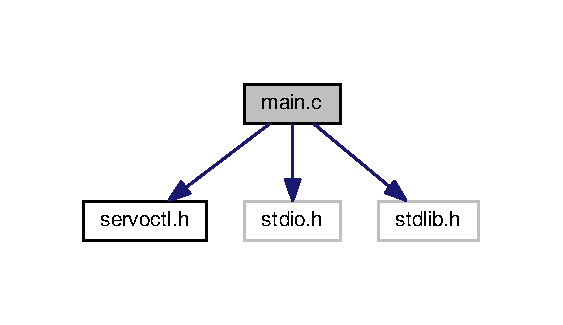
\includegraphics[width=270pt]{main_8c__incl}
\end{center}
\end{figure}
\subsection*{Functions}
\begin{DoxyCompactItemize}
\item 
int \hyperlink{main_8c_a3c04138a5bfe5d72780bb7e82a18e627}{main} (int argc, char $\ast$$\ast$argv)
\end{DoxyCompactItemize}


\subsection{Function Documentation}
\index{main.\+c@{main.\+c}!main@{main}}
\index{main@{main}!main.\+c@{main.\+c}}
\subsubsection[{\texorpdfstring{main(int argc, char $\ast$$\ast$argv)}{main(int argc, char **argv)}}]{\setlength{\rightskip}{0pt plus 5cm}int main (
\begin{DoxyParamCaption}
\item[{int}]{argc, }
\item[{char $\ast$$\ast$}]{argv}
\end{DoxyParamCaption}
)}\hypertarget{main_8c_a3c04138a5bfe5d72780bb7e82a18e627}{}\label{main_8c_a3c04138a5bfe5d72780bb7e82a18e627}

\hypertarget{matrix_8c}{}\section{matrix.\+c File Reference}
\label{matrix_8c}\index{matrix.\+c@{matrix.\+c}}
{\ttfamily \#include $<$stdio.\+h$>$}\\*
{\ttfamily \#include $<$stdlib.\+h$>$}\\*
{\ttfamily \#include $<$stdarg.\+h$>$}\\*
{\ttfamily \#include $<$assert.\+h$>$}\\*
{\ttfamily \#include $<$math.\+h$>$}\\*
{\ttfamily \#include \char`\"{}matrix.\+h\char`\"{}}\\*
Include dependency graph for matrix.\+c\+:\nopagebreak
\begin{figure}[H]
\begin{center}
\leavevmode
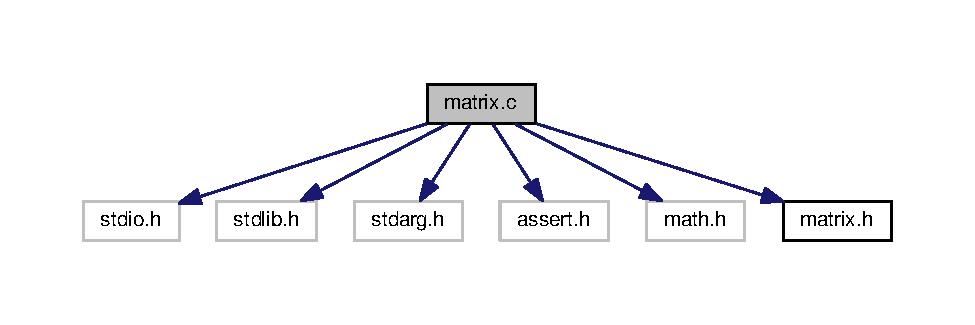
\includegraphics[width=350pt]{matrix_8c__incl}
\end{center}
\end{figure}
\subsection*{Functions}
\begin{DoxyCompactItemize}
\item 
\hyperlink{matrix_8h_a423f7a3e32c1f6d72e65d605ea5e6f5f}{matrix\+\_\+t} $\ast$ \hyperlink{matrix_8c_ada5cab59dea5fc74a2146285abf2e468}{matrix\+\_\+new} (int columns, int rows)
\begin{DoxyCompactList}\small\item\em Create a new matrix. \end{DoxyCompactList}\item 
void \hyperlink{matrix_8c_a8277c0c702668ac9c20d5b4fbbb1c805}{matrix\+\_\+del} (\hyperlink{matrix_8h_a423f7a3e32c1f6d72e65d605ea5e6f5f}{matrix\+\_\+t} $\ast$m)
\begin{DoxyCompactList}\small\item\em Delete a matrix. \end{DoxyCompactList}\item 
\hyperlink{matrix_8h_a423f7a3e32c1f6d72e65d605ea5e6f5f}{matrix\+\_\+t} $\ast$ \hyperlink{matrix_8c_a734238400aafc2b5dbc5cd3d56cd9d60}{matrix\+\_\+get\+\_\+col\+\_\+vector} (\hyperlink{matrix_8h_a423f7a3e32c1f6d72e65d605ea5e6f5f}{matrix\+\_\+t} $\ast$m, int col\+\_\+no)
\begin{DoxyCompactList}\small\item\em Extract a column vector from a matrix. \end{DoxyCompactList}\item 
void \hyperlink{matrix_8c_a2bf3c116d7c23979b805934c18d9d3fd}{matrix\+\_\+set\+\_\+col} (\hyperlink{matrix_8h_a423f7a3e32c1f6d72e65d605ea5e6f5f}{matrix\+\_\+t} $\ast$m, int col\+\_\+no,...)
\begin{DoxyCompactList}\small\item\em Set the column col\+\_\+no in m. \end{DoxyCompactList}\item 
void \hyperlink{matrix_8c_a066269f1cf8e31cee35781be055b541f}{matrix\+\_\+set} (\hyperlink{matrix_8h_a423f7a3e32c1f6d72e65d605ea5e6f5f}{matrix\+\_\+t} $\ast$m, int col, int row, double d)
\begin{DoxyCompactList}\small\item\em Set the element at column col and row row in m to d. \end{DoxyCompactList}\item 
double $\ast$ \hyperlink{matrix_8c_ae6a0f841c360812a20dd2f43a7be3d9e}{matrix\+\_\+get} (\hyperlink{matrix_8h_a423f7a3e32c1f6d72e65d605ea5e6f5f}{matrix\+\_\+t} $\ast$m, int col, int row)
\begin{DoxyCompactList}\small\item\em Return a pointer to the element at col, row in m. \end{DoxyCompactList}\item 
void \hyperlink{matrix_8c_a57c33c823cc314048ff5ffd206a7fd27}{matrix\+\_\+printf} (char $\ast$format, \hyperlink{matrix_8h_a423f7a3e32c1f6d72e65d605ea5e6f5f}{matrix\+\_\+t} $\ast$m)
\begin{DoxyCompactList}\small\item\em Print the contents of matrix m using format. \end{DoxyCompactList}\item 
\hyperlink{matrix_8h_a423f7a3e32c1f6d72e65d605ea5e6f5f}{matrix\+\_\+t} $\ast$ \hyperlink{matrix_8c_af1e14df979d46d4f11464f83f4e6ee22}{matrix\+\_\+rol2r} (\hyperlink{matrix_8h_a423f7a3e32c1f6d72e65d605ea5e6f5f}{matrix\+\_\+t} $\ast$m, double theta)
\begin{DoxyCompactList}\small\item\em Rotate a matrix left (anticlockwise) in 2 dmensions using radians. \end{DoxyCompactList}\item 
\hyperlink{matrix_8h_a423f7a3e32c1f6d72e65d605ea5e6f5f}{matrix\+\_\+t} $\ast$ \hyperlink{matrix_8c_a1e8d8c0421f716763d5bbb5c39af0e5b}{matrix\+\_\+mul} (\hyperlink{matrix_8h_a423f7a3e32c1f6d72e65d605ea5e6f5f}{matrix\+\_\+t} $\ast$m1, \hyperlink{matrix_8h_a423f7a3e32c1f6d72e65d605ea5e6f5f}{matrix\+\_\+t} $\ast$m2)
\begin{DoxyCompactList}\small\item\em multiply m1 x m2 \end{DoxyCompactList}\end{DoxyCompactItemize}


\subsection{Function Documentation}
\index{matrix.\+c@{matrix.\+c}!matrix\+\_\+del@{matrix\+\_\+del}}
\index{matrix\+\_\+del@{matrix\+\_\+del}!matrix.\+c@{matrix.\+c}}
\subsubsection[{\texorpdfstring{matrix\+\_\+del(matrix\+\_\+t $\ast$m)}{matrix_del(matrix_t *m)}}]{\setlength{\rightskip}{0pt plus 5cm}void matrix\+\_\+del (
\begin{DoxyParamCaption}
\item[{{\bf matrix\+\_\+t} $\ast$}]{m}
\end{DoxyParamCaption}
)}\hypertarget{matrix_8c_a8277c0c702668ac9c20d5b4fbbb1c805}{}\label{matrix_8c_a8277c0c702668ac9c20d5b4fbbb1c805}


Delete a matrix. 

\begin{DoxyItemize}
\item m -\/ The matrix to be deleted
\begin{DoxyItemize}
\item Matrices can be created with other functions than \hyperlink{matrix_8c_ada5cab59dea5fc74a2146285abf2e468}{matrix\+\_\+new()}.
\item In general, if the called function returns a pointer to a \hyperlink{matrix_8h_a423f7a3e32c1f6d72e65d605ea5e6f5f}{matrix\+\_\+t}, that matrix must be deleted with this destructor function. 
\end{DoxyItemize}\end{DoxyItemize}
\index{matrix.\+c@{matrix.\+c}!matrix\+\_\+get@{matrix\+\_\+get}}
\index{matrix\+\_\+get@{matrix\+\_\+get}!matrix.\+c@{matrix.\+c}}
\subsubsection[{\texorpdfstring{matrix\+\_\+get(matrix\+\_\+t $\ast$m, int col, int row)}{matrix_get(matrix_t *m, int col, int row)}}]{\setlength{\rightskip}{0pt plus 5cm}double$\ast$ matrix\+\_\+get (
\begin{DoxyParamCaption}
\item[{{\bf matrix\+\_\+t} $\ast$}]{m, }
\item[{int}]{col, }
\item[{int}]{row}
\end{DoxyParamCaption}
)}\hypertarget{matrix_8c_ae6a0f841c360812a20dd2f43a7be3d9e}{}\label{matrix_8c_ae6a0f841c360812a20dd2f43a7be3d9e}


Return a pointer to the element at col, row in m. 


\begin{DoxyItemize}
\item The array containing this element is maintained by matrix\+\_\+t, so don\textquotesingle{}t try to delete this. 
\end{DoxyItemize}\index{matrix.\+c@{matrix.\+c}!matrix\+\_\+get\+\_\+col\+\_\+vector@{matrix\+\_\+get\+\_\+col\+\_\+vector}}
\index{matrix\+\_\+get\+\_\+col\+\_\+vector@{matrix\+\_\+get\+\_\+col\+\_\+vector}!matrix.\+c@{matrix.\+c}}
\subsubsection[{\texorpdfstring{matrix\+\_\+get\+\_\+col\+\_\+vector(matrix\+\_\+t $\ast$m, int col\+\_\+no)}{matrix_get_col_vector(matrix_t *m, int col_no)}}]{\setlength{\rightskip}{0pt plus 5cm}{\bf matrix\+\_\+t}$\ast$ matrix\+\_\+get\+\_\+col\+\_\+vector (
\begin{DoxyParamCaption}
\item[{{\bf matrix\+\_\+t} $\ast$}]{m, }
\item[{int}]{col\+\_\+no}
\end{DoxyParamCaption}
)}\hypertarget{matrix_8c_a734238400aafc2b5dbc5cd3d56cd9d60}{}\label{matrix_8c_a734238400aafc2b5dbc5cd3d56cd9d60}


Extract a column vector from a matrix. 

\begin{DoxyItemize}
\item m -\/ The matrix from which to extract the column \item col\+\_\+no -\/ The column number to extract. Starts with 0. \begin{DoxyReturn}{Returns}
A new vector of type \hyperlink{matrix_8h_a423f7a3e32c1f6d72e65d605ea5e6f5f}{matrix\+\_\+t} that must be deleted with \hyperlink{matrix_8c_a8277c0c702668ac9c20d5b4fbbb1c805}{matrix\+\_\+del()}. 
\end{DoxyReturn}
\end{DoxyItemize}
\index{matrix.\+c@{matrix.\+c}!matrix\+\_\+mul@{matrix\+\_\+mul}}
\index{matrix\+\_\+mul@{matrix\+\_\+mul}!matrix.\+c@{matrix.\+c}}
\subsubsection[{\texorpdfstring{matrix\+\_\+mul(matrix\+\_\+t $\ast$m1, matrix\+\_\+t $\ast$m2)}{matrix_mul(matrix_t *m1, matrix_t *m2)}}]{\setlength{\rightskip}{0pt plus 5cm}{\bf matrix\+\_\+t}$\ast$ matrix\+\_\+mul (
\begin{DoxyParamCaption}
\item[{{\bf matrix\+\_\+t} $\ast$}]{m1, }
\item[{{\bf matrix\+\_\+t} $\ast$}]{m2}
\end{DoxyParamCaption}
)}\hypertarget{matrix_8c_a1e8d8c0421f716763d5bbb5c39af0e5b}{}\label{matrix_8c_a1e8d8c0421f716763d5bbb5c39af0e5b}


multiply m1 x m2 


\begin{DoxyItemize}
\item This function is used as a \textquotesingle{}workhorse\textquotesingle{} for kinematic functions.
\item The result must be deleted with \hyperlink{matrix_8c_a8277c0c702668ac9c20d5b4fbbb1c805}{matrix\+\_\+del()}. \begin{DoxyReturn}{Returns}
A new matrix that must be deleted with \hyperlink{matrix_8c_a8277c0c702668ac9c20d5b4fbbb1c805}{matrix\+\_\+del()}. 
\end{DoxyReturn}

\end{DoxyItemize}\index{matrix.\+c@{matrix.\+c}!matrix\+\_\+new@{matrix\+\_\+new}}
\index{matrix\+\_\+new@{matrix\+\_\+new}!matrix.\+c@{matrix.\+c}}
\subsubsection[{\texorpdfstring{matrix\+\_\+new(int columns, int rows)}{matrix_new(int columns, int rows)}}]{\setlength{\rightskip}{0pt plus 5cm}{\bf matrix\+\_\+t}$\ast$ matrix\+\_\+new (
\begin{DoxyParamCaption}
\item[{int}]{columns, }
\item[{int}]{rows}
\end{DoxyParamCaption}
)}\hypertarget{matrix_8c_ada5cab59dea5fc74a2146285abf2e468}{}\label{matrix_8c_ada5cab59dea5fc74a2146285abf2e468}


Create a new matrix. 

\begin{DoxyItemize}
\item columns -\/ The number of columns in the matrix \item rows -\/ The number of rows in the matrix. \begin{DoxyReturn}{Returns}
A new matric that must be deleted with \hyperlink{matrix_8c_a8277c0c702668ac9c20d5b4fbbb1c805}{matrix\+\_\+del()}. 
\end{DoxyReturn}
\begin{DoxyWarning}{Warning}
Don\textquotesingle{}t free() instances of \hyperlink{matrix_8h_a423f7a3e32c1f6d72e65d605ea5e6f5f}{matrix\+\_\+t}. You\textquotesingle{}ll be leaving dangling pointers inside. 
\end{DoxyWarning}
\end{DoxyItemize}
\index{matrix.\+c@{matrix.\+c}!matrix\+\_\+printf@{matrix\+\_\+printf}}
\index{matrix\+\_\+printf@{matrix\+\_\+printf}!matrix.\+c@{matrix.\+c}}
\subsubsection[{\texorpdfstring{matrix\+\_\+printf(char $\ast$format, matrix\+\_\+t $\ast$m)}{matrix_printf(char *format, matrix_t *m)}}]{\setlength{\rightskip}{0pt plus 5cm}void matrix\+\_\+printf (
\begin{DoxyParamCaption}
\item[{char $\ast$}]{format, }
\item[{{\bf matrix\+\_\+t} $\ast$}]{m}
\end{DoxyParamCaption}
)}\hypertarget{matrix_8c_a57c33c823cc314048ff5ffd206a7fd27}{}\label{matrix_8c_a57c33c823cc314048ff5ffd206a7fd27}


Print the contents of matrix m using format. 

\begin{DoxyItemize}
\item format -\/ Passed on to printf(). \item m -\/ The matrix to print.
\begin{DoxyItemize}
\item Typically, you\textquotesingle{}d use \char`\"{}\%2.\+1f \char`\"{} (note the space). 
\end{DoxyItemize}\end{DoxyItemize}
\index{matrix.\+c@{matrix.\+c}!matrix\+\_\+rol2r@{matrix\+\_\+rol2r}}
\index{matrix\+\_\+rol2r@{matrix\+\_\+rol2r}!matrix.\+c@{matrix.\+c}}
\subsubsection[{\texorpdfstring{matrix\+\_\+rol2r(matrix\+\_\+t $\ast$m, double theta)}{matrix_rol2r(matrix_t *m, double theta)}}]{\setlength{\rightskip}{0pt plus 5cm}{\bf matrix\+\_\+t}$\ast$ matrix\+\_\+rol2r (
\begin{DoxyParamCaption}
\item[{{\bf matrix\+\_\+t} $\ast$}]{m, }
\item[{double}]{theta}
\end{DoxyParamCaption}
)}\hypertarget{matrix_8c_af1e14df979d46d4f11464f83f4e6ee22}{}\label{matrix_8c_af1e14df979d46d4f11464f83f4e6ee22}


Rotate a matrix left (anticlockwise) in 2 dmensions using radians. 


\begin{DoxyItemize}
\item The result must be deleted with \hyperlink{matrix_8c_a8277c0c702668ac9c20d5b4fbbb1c805}{matrix\+\_\+del()}\+: 
\end{DoxyItemize}\index{matrix.\+c@{matrix.\+c}!matrix\+\_\+set@{matrix\+\_\+set}}
\index{matrix\+\_\+set@{matrix\+\_\+set}!matrix.\+c@{matrix.\+c}}
\subsubsection[{\texorpdfstring{matrix\+\_\+set(matrix\+\_\+t $\ast$m, int col, int row, double d)}{matrix_set(matrix_t *m, int col, int row, double d)}}]{\setlength{\rightskip}{0pt plus 5cm}void matrix\+\_\+set (
\begin{DoxyParamCaption}
\item[{{\bf matrix\+\_\+t} $\ast$}]{m, }
\item[{int}]{col, }
\item[{int}]{row, }
\item[{double}]{d}
\end{DoxyParamCaption}
)}\hypertarget{matrix_8c_a066269f1cf8e31cee35781be055b541f}{}\label{matrix_8c_a066269f1cf8e31cee35781be055b541f}


Set the element at column col and row row in m to d. 

-\/\+Same as E\+LM the macro hack, but a lot safer. \index{matrix.\+c@{matrix.\+c}!matrix\+\_\+set\+\_\+col@{matrix\+\_\+set\+\_\+col}}
\index{matrix\+\_\+set\+\_\+col@{matrix\+\_\+set\+\_\+col}!matrix.\+c@{matrix.\+c}}
\subsubsection[{\texorpdfstring{matrix\+\_\+set\+\_\+col(matrix\+\_\+t $\ast$m, int col\+\_\+no,...)}{matrix_set_col(matrix_t *m, int col_no,...)}}]{\setlength{\rightskip}{0pt plus 5cm}void matrix\+\_\+set\+\_\+col (
\begin{DoxyParamCaption}
\item[{{\bf matrix\+\_\+t} $\ast$}]{m, }
\item[{int}]{col\+\_\+no, }
\item[{}]{...}
\end{DoxyParamCaption}
)}\hypertarget{matrix_8c_a2bf3c116d7c23979b805934c18d9d3fd}{}\label{matrix_8c_a2bf3c116d7c23979b805934c18d9d3fd}


Set the column col\+\_\+no in m. 

\begin{DoxyItemize}
\item m -\/ The matrix to maniplulate. \item col\+\_\+no -\/ The column that we wish to set \item ... -\/ The values
\begin{DoxyItemize}
\item The argument list must contain one entry for each rown in m.
\item There is no way to check this without cluttering up the code. 
\end{DoxyItemize}\end{DoxyItemize}

\hypertarget{matrix_8h}{}\section{matrix.\+h File Reference}
\label{matrix_8h}\index{matrix.\+h@{matrix.\+h}}
This graph shows which files directly or indirectly include this file\+:\nopagebreak
\begin{figure}[H]
\begin{center}
\leavevmode
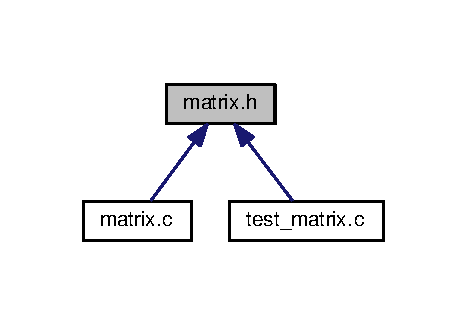
\includegraphics[width=224pt]{matrix_8h__dep__incl}
\end{center}
\end{figure}
\subsection*{Data Structures}
\begin{DoxyCompactItemize}
\item 
struct \hyperlink{structmatrix}{matrix}
\end{DoxyCompactItemize}
\subsection*{Macros}
\begin{DoxyCompactItemize}
\item 
\#define \hyperlink{matrix_8h_aaf4919968b31b42a399d749719bbe126}{E\+LM}(m,  col,  row)~(m-\/$>$v\mbox{[}(m-\/$>$ncols$\ast$row)+col\mbox{]})
\end{DoxyCompactItemize}
\subsection*{Typedefs}
\begin{DoxyCompactItemize}
\item 
typedef struct \hyperlink{structmatrix}{matrix} \hyperlink{matrix_8h_a423f7a3e32c1f6d72e65d605ea5e6f5f}{matrix\+\_\+t}
\end{DoxyCompactItemize}
\subsection*{Functions}
\begin{DoxyCompactItemize}
\item 
\hyperlink{matrix_8h_a423f7a3e32c1f6d72e65d605ea5e6f5f}{matrix\+\_\+t} $\ast$ \hyperlink{matrix_8h_ada5cab59dea5fc74a2146285abf2e468}{matrix\+\_\+new} (int columns, int rows)
\begin{DoxyCompactList}\small\item\em Create a new matrix. \end{DoxyCompactList}\item 
void \hyperlink{matrix_8h_a8277c0c702668ac9c20d5b4fbbb1c805}{matrix\+\_\+del} (\hyperlink{matrix_8h_a423f7a3e32c1f6d72e65d605ea5e6f5f}{matrix\+\_\+t} $\ast$m)
\begin{DoxyCompactList}\small\item\em Delete a matrix. \end{DoxyCompactList}\item 
\hyperlink{matrix_8h_a423f7a3e32c1f6d72e65d605ea5e6f5f}{matrix\+\_\+t} $\ast$ \hyperlink{matrix_8h_a734238400aafc2b5dbc5cd3d56cd9d60}{matrix\+\_\+get\+\_\+col\+\_\+vector} (\hyperlink{matrix_8h_a423f7a3e32c1f6d72e65d605ea5e6f5f}{matrix\+\_\+t} $\ast$m, int col\+\_\+no)
\begin{DoxyCompactList}\small\item\em Extract a column vector from a matrix. \end{DoxyCompactList}\item 
void \hyperlink{matrix_8h_a2bf3c116d7c23979b805934c18d9d3fd}{matrix\+\_\+set\+\_\+col} (\hyperlink{matrix_8h_a423f7a3e32c1f6d72e65d605ea5e6f5f}{matrix\+\_\+t} $\ast$m, int col\+\_\+no,...)
\begin{DoxyCompactList}\small\item\em Set the column col\+\_\+no in m. \end{DoxyCompactList}\item 
\hyperlink{matrix_8h_a423f7a3e32c1f6d72e65d605ea5e6f5f}{matrix\+\_\+t} $\ast$ \hyperlink{matrix_8h_a1e8d8c0421f716763d5bbb5c39af0e5b}{matrix\+\_\+mul} (\hyperlink{matrix_8h_a423f7a3e32c1f6d72e65d605ea5e6f5f}{matrix\+\_\+t} $\ast$m1, \hyperlink{matrix_8h_a423f7a3e32c1f6d72e65d605ea5e6f5f}{matrix\+\_\+t} $\ast$m2)
\begin{DoxyCompactList}\small\item\em multiply m1 x m2 \end{DoxyCompactList}\item 
void \hyperlink{matrix_8h_a6e2e142638d18a26b372e1fe1ad719f4}{matrix\+\_\+set} (\hyperlink{matrix_8h_a423f7a3e32c1f6d72e65d605ea5e6f5f}{matrix\+\_\+t} $\ast$m, int col, int row, double v)
\begin{DoxyCompactList}\small\item\em Set the element at column col and row row in m to d. \end{DoxyCompactList}\item 
double $\ast$ \hyperlink{matrix_8h_ae6a0f841c360812a20dd2f43a7be3d9e}{matrix\+\_\+get} (\hyperlink{matrix_8h_a423f7a3e32c1f6d72e65d605ea5e6f5f}{matrix\+\_\+t} $\ast$m, int col, int row)
\begin{DoxyCompactList}\small\item\em Return a pointer to the element at col, row in m. \end{DoxyCompactList}\item 
void \hyperlink{matrix_8h_a57c33c823cc314048ff5ffd206a7fd27}{matrix\+\_\+printf} (char $\ast$format, \hyperlink{matrix_8h_a423f7a3e32c1f6d72e65d605ea5e6f5f}{matrix\+\_\+t} $\ast$m)
\begin{DoxyCompactList}\small\item\em Print the contents of matrix m using format. \end{DoxyCompactList}\item 
\hyperlink{matrix_8h_a423f7a3e32c1f6d72e65d605ea5e6f5f}{matrix\+\_\+t} $\ast$ \hyperlink{matrix_8h_af1e14df979d46d4f11464f83f4e6ee22}{matrix\+\_\+rol2r} (\hyperlink{matrix_8h_a423f7a3e32c1f6d72e65d605ea5e6f5f}{matrix\+\_\+t} $\ast$m, double theta)
\begin{DoxyCompactList}\small\item\em Rotate a matrix left (anticlockwise) in 2 dmensions using radians. \end{DoxyCompactList}\end{DoxyCompactItemize}


\subsection{Macro Definition Documentation}
\index{matrix.\+h@{matrix.\+h}!E\+LM@{E\+LM}}
\index{E\+LM@{E\+LM}!matrix.\+h@{matrix.\+h}}
\subsubsection[{\texorpdfstring{E\+LM}{ELM}}]{\setlength{\rightskip}{0pt plus 5cm}\#define E\+LM(
\begin{DoxyParamCaption}
\item[{}]{m, }
\item[{}]{col, }
\item[{}]{row}
\end{DoxyParamCaption}
)~(m-\/$>$v\mbox{[}(m-\/$>$ncols$\ast$row)+col\mbox{]})}\hypertarget{matrix_8h_aaf4919968b31b42a399d749719bbe126}{}\label{matrix_8h_aaf4919968b31b42a399d749719bbe126}


\subsection{Typedef Documentation}
\index{matrix.\+h@{matrix.\+h}!matrix\+\_\+t@{matrix\+\_\+t}}
\index{matrix\+\_\+t@{matrix\+\_\+t}!matrix.\+h@{matrix.\+h}}
\subsubsection[{\texorpdfstring{matrix\+\_\+t}{matrix_t}}]{\setlength{\rightskip}{0pt plus 5cm}typedef struct {\bf matrix}  {\bf matrix\+\_\+t}}\hypertarget{matrix_8h_a423f7a3e32c1f6d72e65d605ea5e6f5f}{}\label{matrix_8h_a423f7a3e32c1f6d72e65d605ea5e6f5f}


\subsection{Function Documentation}
\index{matrix.\+h@{matrix.\+h}!matrix\+\_\+del@{matrix\+\_\+del}}
\index{matrix\+\_\+del@{matrix\+\_\+del}!matrix.\+h@{matrix.\+h}}
\subsubsection[{\texorpdfstring{matrix\+\_\+del(matrix\+\_\+t $\ast$m)}{matrix_del(matrix_t *m)}}]{\setlength{\rightskip}{0pt plus 5cm}void matrix\+\_\+del (
\begin{DoxyParamCaption}
\item[{{\bf matrix\+\_\+t} $\ast$}]{m}
\end{DoxyParamCaption}
)}\hypertarget{matrix_8h_a8277c0c702668ac9c20d5b4fbbb1c805}{}\label{matrix_8h_a8277c0c702668ac9c20d5b4fbbb1c805}


Delete a matrix. 

\begin{DoxyItemize}
\item m -\/ The matrix to be deleted
\begin{DoxyItemize}
\item Matrices can be created with other functions than \hyperlink{matrix_8c_ada5cab59dea5fc74a2146285abf2e468}{matrix\+\_\+new()}.
\item In general, if the called function returns a pointer to a \hyperlink{matrix_8h_a423f7a3e32c1f6d72e65d605ea5e6f5f}{matrix\+\_\+t}, that matrix must be deleted with this destructor function. 
\end{DoxyItemize}\end{DoxyItemize}
\index{matrix.\+h@{matrix.\+h}!matrix\+\_\+get@{matrix\+\_\+get}}
\index{matrix\+\_\+get@{matrix\+\_\+get}!matrix.\+h@{matrix.\+h}}
\subsubsection[{\texorpdfstring{matrix\+\_\+get(matrix\+\_\+t $\ast$m, int col, int row)}{matrix_get(matrix_t *m, int col, int row)}}]{\setlength{\rightskip}{0pt plus 5cm}double$\ast$ matrix\+\_\+get (
\begin{DoxyParamCaption}
\item[{{\bf matrix\+\_\+t} $\ast$}]{m, }
\item[{int}]{col, }
\item[{int}]{row}
\end{DoxyParamCaption}
)}\hypertarget{matrix_8h_ae6a0f841c360812a20dd2f43a7be3d9e}{}\label{matrix_8h_ae6a0f841c360812a20dd2f43a7be3d9e}


Return a pointer to the element at col, row in m. 


\begin{DoxyItemize}
\item The array containing this element is maintained by matrix\+\_\+t, so don\textquotesingle{}t try to delete this. 
\end{DoxyItemize}\index{matrix.\+h@{matrix.\+h}!matrix\+\_\+get\+\_\+col\+\_\+vector@{matrix\+\_\+get\+\_\+col\+\_\+vector}}
\index{matrix\+\_\+get\+\_\+col\+\_\+vector@{matrix\+\_\+get\+\_\+col\+\_\+vector}!matrix.\+h@{matrix.\+h}}
\subsubsection[{\texorpdfstring{matrix\+\_\+get\+\_\+col\+\_\+vector(matrix\+\_\+t $\ast$m, int col\+\_\+no)}{matrix_get_col_vector(matrix_t *m, int col_no)}}]{\setlength{\rightskip}{0pt plus 5cm}{\bf matrix\+\_\+t}$\ast$ matrix\+\_\+get\+\_\+col\+\_\+vector (
\begin{DoxyParamCaption}
\item[{{\bf matrix\+\_\+t} $\ast$}]{m, }
\item[{int}]{col\+\_\+no}
\end{DoxyParamCaption}
)}\hypertarget{matrix_8h_a734238400aafc2b5dbc5cd3d56cd9d60}{}\label{matrix_8h_a734238400aafc2b5dbc5cd3d56cd9d60}


Extract a column vector from a matrix. 

\begin{DoxyItemize}
\item m -\/ The matrix from which to extract the column \item col\+\_\+no -\/ The column number to extract. Starts with 0. \begin{DoxyReturn}{Returns}
A new vector of type \hyperlink{matrix_8h_a423f7a3e32c1f6d72e65d605ea5e6f5f}{matrix\+\_\+t} that must be deleted with \hyperlink{matrix_8c_a8277c0c702668ac9c20d5b4fbbb1c805}{matrix\+\_\+del()}. 
\end{DoxyReturn}
\end{DoxyItemize}
\index{matrix.\+h@{matrix.\+h}!matrix\+\_\+mul@{matrix\+\_\+mul}}
\index{matrix\+\_\+mul@{matrix\+\_\+mul}!matrix.\+h@{matrix.\+h}}
\subsubsection[{\texorpdfstring{matrix\+\_\+mul(matrix\+\_\+t $\ast$m1, matrix\+\_\+t $\ast$m2)}{matrix_mul(matrix_t *m1, matrix_t *m2)}}]{\setlength{\rightskip}{0pt plus 5cm}{\bf matrix\+\_\+t}$\ast$ matrix\+\_\+mul (
\begin{DoxyParamCaption}
\item[{{\bf matrix\+\_\+t} $\ast$}]{m1, }
\item[{{\bf matrix\+\_\+t} $\ast$}]{m2}
\end{DoxyParamCaption}
)}\hypertarget{matrix_8h_a1e8d8c0421f716763d5bbb5c39af0e5b}{}\label{matrix_8h_a1e8d8c0421f716763d5bbb5c39af0e5b}


multiply m1 x m2 


\begin{DoxyItemize}
\item This function is used as a \textquotesingle{}workhorse\textquotesingle{} for kinematic functions.
\item The result must be deleted with \hyperlink{matrix_8c_a8277c0c702668ac9c20d5b4fbbb1c805}{matrix\+\_\+del()}. \begin{DoxyReturn}{Returns}
A new matrix that must be deleted with \hyperlink{matrix_8c_a8277c0c702668ac9c20d5b4fbbb1c805}{matrix\+\_\+del()}. 
\end{DoxyReturn}

\end{DoxyItemize}\index{matrix.\+h@{matrix.\+h}!matrix\+\_\+new@{matrix\+\_\+new}}
\index{matrix\+\_\+new@{matrix\+\_\+new}!matrix.\+h@{matrix.\+h}}
\subsubsection[{\texorpdfstring{matrix\+\_\+new(int columns, int rows)}{matrix_new(int columns, int rows)}}]{\setlength{\rightskip}{0pt plus 5cm}{\bf matrix\+\_\+t}$\ast$ matrix\+\_\+new (
\begin{DoxyParamCaption}
\item[{int}]{columns, }
\item[{int}]{rows}
\end{DoxyParamCaption}
)}\hypertarget{matrix_8h_ada5cab59dea5fc74a2146285abf2e468}{}\label{matrix_8h_ada5cab59dea5fc74a2146285abf2e468}


Create a new matrix. 

\begin{DoxyItemize}
\item columns -\/ The number of columns in the matrix \item rows -\/ The number of rows in the matrix. \begin{DoxyReturn}{Returns}
A new matric that must be deleted with \hyperlink{matrix_8c_a8277c0c702668ac9c20d5b4fbbb1c805}{matrix\+\_\+del()}. 
\end{DoxyReturn}
\begin{DoxyWarning}{Warning}
Don\textquotesingle{}t free() instances of \hyperlink{matrix_8h_a423f7a3e32c1f6d72e65d605ea5e6f5f}{matrix\+\_\+t}. You\textquotesingle{}ll be leaving dangling pointers inside. 
\end{DoxyWarning}
\end{DoxyItemize}
\index{matrix.\+h@{matrix.\+h}!matrix\+\_\+printf@{matrix\+\_\+printf}}
\index{matrix\+\_\+printf@{matrix\+\_\+printf}!matrix.\+h@{matrix.\+h}}
\subsubsection[{\texorpdfstring{matrix\+\_\+printf(char $\ast$format, matrix\+\_\+t $\ast$m)}{matrix_printf(char *format, matrix_t *m)}}]{\setlength{\rightskip}{0pt plus 5cm}void matrix\+\_\+printf (
\begin{DoxyParamCaption}
\item[{char $\ast$}]{format, }
\item[{{\bf matrix\+\_\+t} $\ast$}]{m}
\end{DoxyParamCaption}
)}\hypertarget{matrix_8h_a57c33c823cc314048ff5ffd206a7fd27}{}\label{matrix_8h_a57c33c823cc314048ff5ffd206a7fd27}


Print the contents of matrix m using format. 

\begin{DoxyItemize}
\item format -\/ Passed on to printf(). \item m -\/ The matrix to print.
\begin{DoxyItemize}
\item Typically, you\textquotesingle{}d use \char`\"{}\%2.\+1f \char`\"{} (note the space). 
\end{DoxyItemize}\end{DoxyItemize}
\index{matrix.\+h@{matrix.\+h}!matrix\+\_\+rol2r@{matrix\+\_\+rol2r}}
\index{matrix\+\_\+rol2r@{matrix\+\_\+rol2r}!matrix.\+h@{matrix.\+h}}
\subsubsection[{\texorpdfstring{matrix\+\_\+rol2r(matrix\+\_\+t $\ast$m, double theta)}{matrix_rol2r(matrix_t *m, double theta)}}]{\setlength{\rightskip}{0pt plus 5cm}{\bf matrix\+\_\+t}$\ast$ matrix\+\_\+rol2r (
\begin{DoxyParamCaption}
\item[{{\bf matrix\+\_\+t} $\ast$}]{m, }
\item[{double}]{theta}
\end{DoxyParamCaption}
)}\hypertarget{matrix_8h_af1e14df979d46d4f11464f83f4e6ee22}{}\label{matrix_8h_af1e14df979d46d4f11464f83f4e6ee22}


Rotate a matrix left (anticlockwise) in 2 dmensions using radians. 


\begin{DoxyItemize}
\item The result must be deleted with \hyperlink{matrix_8c_a8277c0c702668ac9c20d5b4fbbb1c805}{matrix\+\_\+del()}\+: 
\end{DoxyItemize}\index{matrix.\+h@{matrix.\+h}!matrix\+\_\+set@{matrix\+\_\+set}}
\index{matrix\+\_\+set@{matrix\+\_\+set}!matrix.\+h@{matrix.\+h}}
\subsubsection[{\texorpdfstring{matrix\+\_\+set(matrix\+\_\+t $\ast$m, int col, int row, double v)}{matrix_set(matrix_t *m, int col, int row, double v)}}]{\setlength{\rightskip}{0pt plus 5cm}void matrix\+\_\+set (
\begin{DoxyParamCaption}
\item[{{\bf matrix\+\_\+t} $\ast$}]{m, }
\item[{int}]{col, }
\item[{int}]{row, }
\item[{double}]{d}
\end{DoxyParamCaption}
)}\hypertarget{matrix_8h_a6e2e142638d18a26b372e1fe1ad719f4}{}\label{matrix_8h_a6e2e142638d18a26b372e1fe1ad719f4}


Set the element at column col and row row in m to d. 

-\/\+Same as E\+LM the macro hack, but a lot safer. \index{matrix.\+h@{matrix.\+h}!matrix\+\_\+set\+\_\+col@{matrix\+\_\+set\+\_\+col}}
\index{matrix\+\_\+set\+\_\+col@{matrix\+\_\+set\+\_\+col}!matrix.\+h@{matrix.\+h}}
\subsubsection[{\texorpdfstring{matrix\+\_\+set\+\_\+col(matrix\+\_\+t $\ast$m, int col\+\_\+no,...)}{matrix_set_col(matrix_t *m, int col_no,...)}}]{\setlength{\rightskip}{0pt plus 5cm}void matrix\+\_\+set\+\_\+col (
\begin{DoxyParamCaption}
\item[{{\bf matrix\+\_\+t} $\ast$}]{m, }
\item[{int}]{col\+\_\+no, }
\item[{}]{...}
\end{DoxyParamCaption}
)}\hypertarget{matrix_8h_a2bf3c116d7c23979b805934c18d9d3fd}{}\label{matrix_8h_a2bf3c116d7c23979b805934c18d9d3fd}


Set the column col\+\_\+no in m. 

\begin{DoxyItemize}
\item m -\/ The matrix to maniplulate. \item col\+\_\+no -\/ The column that we wish to set \item ... -\/ The values
\begin{DoxyItemize}
\item The argument list must contain one entry for each rown in m.
\item There is no way to check this without cluttering up the code. 
\end{DoxyItemize}\end{DoxyItemize}

\hypertarget{_r_e_a_d_m_e_8md}{}\section{R\+E\+A\+D\+M\+E.\+md File Reference}
\label{_r_e_a_d_m_e_8md}\index{R\+E\+A\+D\+M\+E.\+md@{R\+E\+A\+D\+M\+E.\+md}}

\hypertarget{servocontrol_8c}{}\section{servocontrol.\+c File Reference}
\label{servocontrol_8c}\index{servocontrol.\+c@{servocontrol.\+c}}
{\ttfamily \#include $<$stdio.\+h$>$}\\*
{\ttfamily \#include $<$stdlib.\+h$>$}\\*
{\ttfamily \#include \char`\"{}servoctl.\+h\char`\"{}}\\*
Include dependency graph for servocontrol.\+c\+:\nopagebreak
\begin{figure}[H]
\begin{center}
\leavevmode
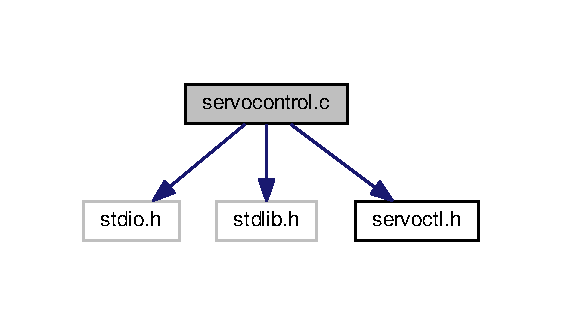
\includegraphics[width=270pt]{servocontrol_8c__incl}
\end{center}
\end{figure}
\subsection*{Functions}
\begin{DoxyCompactItemize}
\item 
int \hyperlink{servocontrol_8c_a3c04138a5bfe5d72780bb7e82a18e627}{main} (int argc, char $\ast$$\ast$argv)
\end{DoxyCompactItemize}


\subsection{Function Documentation}
\index{servocontrol.\+c@{servocontrol.\+c}!main@{main}}
\index{main@{main}!servocontrol.\+c@{servocontrol.\+c}}
\subsubsection[{\texorpdfstring{main(int argc, char $\ast$$\ast$argv)}{main(int argc, char **argv)}}]{\setlength{\rightskip}{0pt plus 5cm}int main (
\begin{DoxyParamCaption}
\item[{int}]{argc, }
\item[{char $\ast$$\ast$}]{argv}
\end{DoxyParamCaption}
)}\hypertarget{servocontrol_8c_a3c04138a5bfe5d72780bb7e82a18e627}{}\label{servocontrol_8c_a3c04138a5bfe5d72780bb7e82a18e627}

\hypertarget{servoctl_8c}{}\section{servoctl.\+c File Reference}
\label{servoctl_8c}\index{servoctl.\+c@{servoctl.\+c}}
{\ttfamily \#include $<$stdio.\+h$>$}\\*
{\ttfamily \#include $<$stdlib.\+h$>$}\\*
Include dependency graph for servoctl.\+c\+:\nopagebreak
\begin{figure}[H]
\begin{center}
\leavevmode
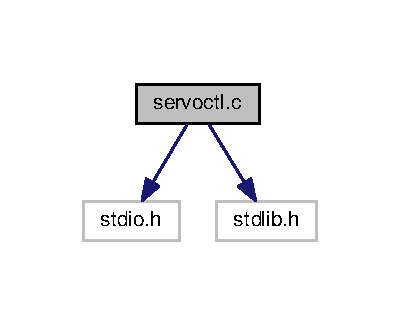
\includegraphics[width=192pt]{servoctl_8c__incl}
\end{center}
\end{figure}
\subsection*{Functions}
\begin{DoxyCompactItemize}
\item 
double $\ast$ \hyperlink{servoctl_8c_ae7a46562f652d66a307a5644f4cd64d5}{interpolate} (double p0, double p1, int numsteps)
\end{DoxyCompactItemize}


\subsection{Function Documentation}
\index{servoctl.\+c@{servoctl.\+c}!interpolate@{interpolate}}
\index{interpolate@{interpolate}!servoctl.\+c@{servoctl.\+c}}
\subsubsection[{\texorpdfstring{interpolate(double p0, double p1, int numsteps)}{interpolate(double p0, double p1, int numsteps)}}]{\setlength{\rightskip}{0pt plus 5cm}double$\ast$ interpolate (
\begin{DoxyParamCaption}
\item[{double}]{p0, }
\item[{double}]{p1, }
\item[{int}]{numsteps}
\end{DoxyParamCaption}
)}\hypertarget{servoctl_8c_ae7a46562f652d66a307a5644f4cd64d5}{}\label{servoctl_8c_ae7a46562f652d66a307a5644f4cd64d5}

\hypertarget{servoctl_8h}{}\section{servoctl.\+h File Reference}
\label{servoctl_8h}\index{servoctl.\+h@{servoctl.\+h}}
This graph shows which files directly or indirectly include this file\+:\nopagebreak
\begin{figure}[H]
\begin{center}
\leavevmode
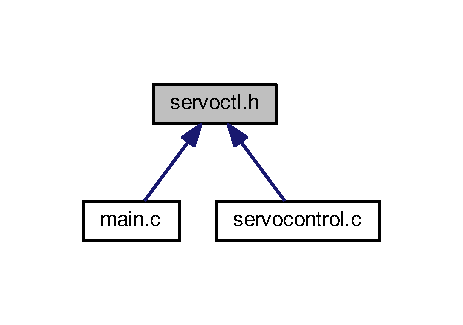
\includegraphics[width=222pt]{servoctl_8h__dep__incl}
\end{center}
\end{figure}
\subsection*{Data Structures}
\begin{DoxyCompactItemize}
\item 
struct \hyperlink{structlinkage}{linkage}
\end{DoxyCompactItemize}
\subsection*{Functions}
\begin{DoxyCompactItemize}
\item 
struct \hyperlink{structlinkage}{linkage} \hyperlink{servoctl_8h_a8403506ff6bd138fd1aab7707e31870d}{interpolate} (double p0, double p1, int numsteps)
\end{DoxyCompactItemize}
\subsection*{Variables}
\begin{DoxyCompactItemize}
\item 
\hyperlink{servoctl_8h_ab7212a9ff1ec58211f1b689374f11766}{base\+\_\+x}
\item 
\hyperlink{servoctl_8h_aed760843bedfbb6de7f205758ef0d49b}{base\+\_\+y}
\end{DoxyCompactItemize}


\subsection{Function Documentation}
\index{servoctl.\+h@{servoctl.\+h}!interpolate@{interpolate}}
\index{interpolate@{interpolate}!servoctl.\+h@{servoctl.\+h}}
\subsubsection[{\texorpdfstring{interpolate(double p0, double p1, int numsteps)}{interpolate(double p0, double p1, int numsteps)}}]{\setlength{\rightskip}{0pt plus 5cm}struct {\bf linkage} interpolate (
\begin{DoxyParamCaption}
\item[{double}]{p0, }
\item[{double}]{p1, }
\item[{int}]{numsteps}
\end{DoxyParamCaption}
)}\hypertarget{servoctl_8h_a8403506ff6bd138fd1aab7707e31870d}{}\label{servoctl_8h_a8403506ff6bd138fd1aab7707e31870d}


\subsection{Variable Documentation}
\index{servoctl.\+h@{servoctl.\+h}!base\+\_\+x@{base\+\_\+x}}
\index{base\+\_\+x@{base\+\_\+x}!servoctl.\+h@{servoctl.\+h}}
\subsubsection[{\texorpdfstring{base\+\_\+x}{base_x}}]{\setlength{\rightskip}{0pt plus 5cm}base\+\_\+x}\hypertarget{servoctl_8h_ab7212a9ff1ec58211f1b689374f11766}{}\label{servoctl_8h_ab7212a9ff1ec58211f1b689374f11766}
\index{servoctl.\+h@{servoctl.\+h}!base\+\_\+y@{base\+\_\+y}}
\index{base\+\_\+y@{base\+\_\+y}!servoctl.\+h@{servoctl.\+h}}
\subsubsection[{\texorpdfstring{base\+\_\+y}{base_y}}]{\setlength{\rightskip}{0pt plus 5cm}base\+\_\+y}\hypertarget{servoctl_8h_aed760843bedfbb6de7f205758ef0d49b}{}\label{servoctl_8h_aed760843bedfbb6de7f205758ef0d49b}

\hypertarget{test__matrix_8c}{}\section{test\+\_\+matrix.\+c File Reference}
\label{test__matrix_8c}\index{test\+\_\+matrix.\+c@{test\+\_\+matrix.\+c}}
{\ttfamily \#include $<$stdio.\+h$>$}\\*
{\ttfamily \#include $<$stdlib.\+h$>$}\\*
{\ttfamily \#include $<$assert.\+h$>$}\\*
{\ttfamily \#include \char`\"{}matrix.\+h\char`\"{}}\\*
Include dependency graph for test\+\_\+matrix.\+c\+:
\nopagebreak
\begin{figure}[H]
\begin{center}
\leavevmode
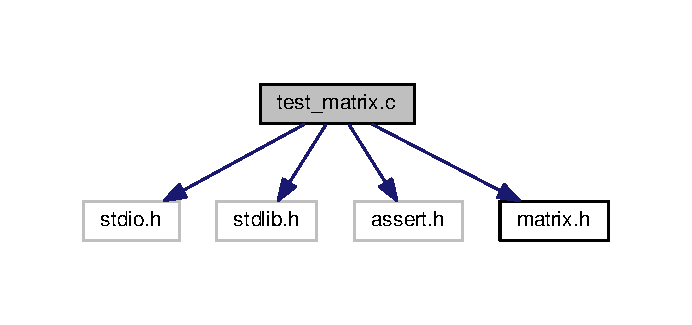
\includegraphics[width=332pt]{test__matrix_8c__incl}
\end{center}
\end{figure}
\subsection*{Macros}
\begin{DoxyCompactItemize}
\item 
\#define \hyperlink{test__matrix_8c_a598a3330b3c21701223ee0ca14316eca}{PI}~3.\+141592654
\end{DoxyCompactItemize}
\subsection*{Functions}
\begin{DoxyCompactItemize}
\item 
void \hyperlink{test__matrix_8c_a0f22b2e88e11fe8ed46b427bd67c178e}{test\+\_\+matrix\+\_\+new} ()
\item 
void \hyperlink{test__matrix_8c_a19198c2ed4c7f6dde90dc28b2fed51f0}{test\+\_\+matrix\+\_\+mul} ()
\item 
void \hyperlink{test__matrix_8c_ab2d8ced00b7f4878853c5e89bed8c434}{test\+\_\+matrix\+\_\+rol} ()
\item 
void \hyperlink{test__matrix_8c_aae5be0cae3fb5ac3cb07946fff70a1b5}{test\+\_\+matrix\+\_\+set\+\_\+col} ()
\item 
void \hyperlink{test__matrix_8c_a8b972c959cb5ce067be1d27de75a1623}{test\+\_\+matrix\+\_\+printf} ()
\item 
int \hyperlink{test__matrix_8c_ae66f6b31b5ad750f1fe042a706a4e3d4}{main} ()
\end{DoxyCompactItemize}


\subsection{Macro Definition Documentation}
\index{test\+\_\+matrix.\+c@{test\+\_\+matrix.\+c}!PI@{PI}}
\index{PI@{PI}!test\+\_\+matrix.\+c@{test\+\_\+matrix.\+c}}
\subsubsection[{\texorpdfstring{PI}{PI}}]{\setlength{\rightskip}{0pt plus 5cm}\#define PI~3.\+141592654}\hypertarget{test__matrix_8c_a598a3330b3c21701223ee0ca14316eca}{}\label{test__matrix_8c_a598a3330b3c21701223ee0ca14316eca}


\subsection{Function Documentation}
\index{test\+\_\+matrix.\+c@{test\+\_\+matrix.\+c}!main@{main}}
\index{main@{main}!test\+\_\+matrix.\+c@{test\+\_\+matrix.\+c}}
\subsubsection[{\texorpdfstring{main()}{main()}}]{\setlength{\rightskip}{0pt plus 5cm}int main (
\begin{DoxyParamCaption}
{}
\end{DoxyParamCaption}
)}\hypertarget{test__matrix_8c_ae66f6b31b5ad750f1fe042a706a4e3d4}{}\label{test__matrix_8c_ae66f6b31b5ad750f1fe042a706a4e3d4}
\index{test\+\_\+matrix.\+c@{test\+\_\+matrix.\+c}!test\+\_\+matrix\+\_\+mul@{test\+\_\+matrix\+\_\+mul}}
\index{test\+\_\+matrix\+\_\+mul@{test\+\_\+matrix\+\_\+mul}!test\+\_\+matrix.\+c@{test\+\_\+matrix.\+c}}
\subsubsection[{\texorpdfstring{test\+\_\+matrix\+\_\+mul()}{test_matrix_mul()}}]{\setlength{\rightskip}{0pt plus 5cm}void test\+\_\+matrix\+\_\+mul (
\begin{DoxyParamCaption}
{}
\end{DoxyParamCaption}
)}\hypertarget{test__matrix_8c_a19198c2ed4c7f6dde90dc28b2fed51f0}{}\label{test__matrix_8c_a19198c2ed4c7f6dde90dc28b2fed51f0}
\index{test\+\_\+matrix.\+c@{test\+\_\+matrix.\+c}!test\+\_\+matrix\+\_\+new@{test\+\_\+matrix\+\_\+new}}
\index{test\+\_\+matrix\+\_\+new@{test\+\_\+matrix\+\_\+new}!test\+\_\+matrix.\+c@{test\+\_\+matrix.\+c}}
\subsubsection[{\texorpdfstring{test\+\_\+matrix\+\_\+new()}{test_matrix_new()}}]{\setlength{\rightskip}{0pt plus 5cm}void test\+\_\+matrix\+\_\+new (
\begin{DoxyParamCaption}
{}
\end{DoxyParamCaption}
)}\hypertarget{test__matrix_8c_a0f22b2e88e11fe8ed46b427bd67c178e}{}\label{test__matrix_8c_a0f22b2e88e11fe8ed46b427bd67c178e}
\index{test\+\_\+matrix.\+c@{test\+\_\+matrix.\+c}!test\+\_\+matrix\+\_\+printf@{test\+\_\+matrix\+\_\+printf}}
\index{test\+\_\+matrix\+\_\+printf@{test\+\_\+matrix\+\_\+printf}!test\+\_\+matrix.\+c@{test\+\_\+matrix.\+c}}
\subsubsection[{\texorpdfstring{test\+\_\+matrix\+\_\+printf()}{test_matrix_printf()}}]{\setlength{\rightskip}{0pt plus 5cm}void test\+\_\+matrix\+\_\+printf (
\begin{DoxyParamCaption}
{}
\end{DoxyParamCaption}
)}\hypertarget{test__matrix_8c_a8b972c959cb5ce067be1d27de75a1623}{}\label{test__matrix_8c_a8b972c959cb5ce067be1d27de75a1623}
\index{test\+\_\+matrix.\+c@{test\+\_\+matrix.\+c}!test\+\_\+matrix\+\_\+rol@{test\+\_\+matrix\+\_\+rol}}
\index{test\+\_\+matrix\+\_\+rol@{test\+\_\+matrix\+\_\+rol}!test\+\_\+matrix.\+c@{test\+\_\+matrix.\+c}}
\subsubsection[{\texorpdfstring{test\+\_\+matrix\+\_\+rol()}{test_matrix_rol()}}]{\setlength{\rightskip}{0pt plus 5cm}void test\+\_\+matrix\+\_\+rol (
\begin{DoxyParamCaption}
{}
\end{DoxyParamCaption}
)}\hypertarget{test__matrix_8c_ab2d8ced00b7f4878853c5e89bed8c434}{}\label{test__matrix_8c_ab2d8ced00b7f4878853c5e89bed8c434}
\index{test\+\_\+matrix.\+c@{test\+\_\+matrix.\+c}!test\+\_\+matrix\+\_\+set\+\_\+col@{test\+\_\+matrix\+\_\+set\+\_\+col}}
\index{test\+\_\+matrix\+\_\+set\+\_\+col@{test\+\_\+matrix\+\_\+set\+\_\+col}!test\+\_\+matrix.\+c@{test\+\_\+matrix.\+c}}
\subsubsection[{\texorpdfstring{test\+\_\+matrix\+\_\+set\+\_\+col()}{test_matrix_set_col()}}]{\setlength{\rightskip}{0pt plus 5cm}void test\+\_\+matrix\+\_\+set\+\_\+col (
\begin{DoxyParamCaption}
{}
\end{DoxyParamCaption}
)}\hypertarget{test__matrix_8c_aae5be0cae3fb5ac3cb07946fff70a1b5}{}\label{test__matrix_8c_aae5be0cae3fb5ac3cb07946fff70a1b5}

%--- End generated contents ---

% Index
\backmatter
\newpage
\phantomsection
\clearemptydoublepage
\addcontentsline{toc}{chapter}{Index}
\printindex

\end{document}
